\documentclass[
  pdftex,
  chapterprefix,
  headsepline,
  footsepline,
  colordvi,
  11pt,
  a4paper,
  halfparskip,
  final,
  appendixprefix,
  bibtotoc]{scrbook}
% uncomment the following line (mutual exclusive to the one above) to enter the draft mode.
%\documentclass[colordvi,11pt,a4paper,halfparskip,draft,appendixprefix,bibtotoc]{scrbook}

%
% neues if definieren, um zwischen PDF und DVI entscheiden zu k�nnen.
%
\usepackage{ifpdf}
\ifx\pdfoutput\undefined
\pdffalse %not PDFLaTeX
\else
\pdfoutput=1
\pdftrue
\fi
%\tracingstats=2
%\usepackage{layout}
% german language support (hyphenation etc)  
\usepackage[english]{babel}

% for prettier tables
\usepackage{booktabs}

% support for latin1 characters. That means you can enter umlauts directly
% no need for "a "u "o "s anymore
\usepackage[utf8x]{inputenc}
%\usepackage[latin1]{inputenc}

% provides the \url{} command to pretty print urls
\usepackage{url}

% needed for a german bibliography-style (s. below)
\usepackage{bibgerm}

% allows text flowing around figures.
\usepackage{wrapfig}

% allows to \includegraphics
\usepackage{graphicx}

% defines some standard colornames like "black" etc.
\usepackage{color}

% allows to color tablecells
\usepackage{colortbl}

% provides an easier interface to if-then-else constructs in 
% custom macros
\usepackage{ifthen}

% allows tables to break over pages.
\usepackage{supertabular}

% allows to have different kinds paper orientations in the same pdf-documnent
\usepackage{pdflscape}

% allows to specify absolute texpos for textboxes. This is generally only important for the titlepage
\usepackage[absolute]{textpos}

% allows to enumerate different figures with a) b) in the same figure-environment.
\usepackage{subfigure}

% finetune the gaps between figure and text in the subfigure environment (basically close the gap as much as possible)
\renewcommand{\subfigtopskip}{0pt}
\renewcommand{\subfigbottomskip}{0pt}

% some color definitions for the pdf statements below
\definecolor{mygrey}{rgb}{0.45,0.45,0.45}
\definecolor{mydarkgrey}{rgb}{0.2,0.2,0.2}
\definecolor{red}{rgb}{1.0,0.33,0.33}
\definecolor{orange}{rgb}{1.00,0.73,0.33}
\definecolor{yellow}{rgb}{0.95,0.92,0.}
\definecolor{lightgreen}{rgb}{0.3,0.95,0.46}
\definecolor{titleblue}{rgb}{0.03,0.10,0.46}

\ifpdf
% Metadata and configuration of the pdf output:
% Do not forget to enter the correct title, author, subject und keywords

% For screen viewing it is nice to have references marked in a slightly different
% color than the rest of the text. Since they will be hyperlinks to the 
% referenced objects.
\usepackage[pdftex,
             pdftitle={},
             colorlinks,
             linkcolor={mydarkgrey},
             citecolor={mygrey},
             urlcolor={black},
             plainpages={false},
             bookmarksnumbered={true},
             pdfauthor={},
             pdfsubject={},
             pdfkeywords={},
             pdfstartview={FitBH}]{hyperref}

% For the final printouts (remember - you need at least three - one for each examiner and one for the archive 
% [ This might have changed - so contact the "Pr�fungsamt" about the current regulations !! ] - it is better
% to have all text in the same color (namely black).
% 
%\usepackage[pdftex,
%            pdftitle={},
%            colorlinks,
%            linkcolor={black},
%            citecolor={black},
%            urlcolor={black},
%            plainpages={false},
%            bookmarksnumbered={true},
%            pdfauthor={},
%            pdfsubject={},
%            pdfkeywords={},
%            pdfstartview={FitBH}]{hyperref}
\pdfcompresslevel=9
\fi

% some configuration for the amount of text on a single page
\usepackage{typearea}
\areaset[1.5cm]{418pt}{658pt}
\setlength{\headheight}{37pt}

% Enter author and title for the titlepage.
\author{}
\title{}

% To avoid nasty mistakes like having comments directly in the textflow
% the following \todo macro was defined. With that you can enter
% \todo{What I still have to do here} 
% inside of your text and a marker will appear at the page's margin with the 
% text "What I still have to do here".
% The first line activates this feature. If you comment it out and uncomment
% the second line below there will be no error messages and no todos will be shown
% anymore. So - even if you have forgotten to delete one of them - they will not appear
% in the final printout. 
\newcommand{\todo}[1]{\marginpar{\textcolor{red}{ToDo:} #1}}
%\newcommand{\todo}[1]{}

% We recommend to split your document into several files. Usually one for every chapter is a 
% good idea. If you follow this guideline (how to assemble these files in a single document
% see two paragraphs below) you will be able to single out chapters via the \includeonly{}
% command. Using this mechanism page numbering and references of the full run before will be
% preserved. This also nice, if your latex run tends to get slow and you need to fine tune 
% some formatting in one chapter - just include that one. The rest (or at least the ones before
% the one currently under construction) will remain untouched. This means a boost in compilation time.
%\includeonly{chapter2}

\begin{document}
% the next two lines influence the detailedness of the table of contents
% and to what structure depth numbers are written before sections/subsections/paragraphs
% You should not touch this
\setcounter{tocdepth}{2}
\setcounter{secnumdepth}{3}
\frontmatter
% here the titlepage is included. Look into the file "titlePage.tex" to 
% adapt it to your needs (name, title etc.)
% %!TEX root=../../Vorname_Nachname_Diplomarbeit.tex

% Titelseite braucht folgenden  Eintrag
% \usepackage[absolute]{textpos}
% textpos ist nicht Bestandteil von tetex
% kann aber von dante heruntergeladen werden
\begin{titlepage}
\vspace*{-1cm}
\newlength{\links}
\setlength{\links}{0.9cm}
\setlength{\TPHorizModule}{1cm}
\setlength{\TPVertModule}{1cm}
\textblockorigin{0pt}{0pt}

\sf
\LARGE

\begin{textblock}{16.5}(2.8,2.6)
 \hspace*{-0.25cm} \textbf{UNIVERSITÄT DUISBURG-ESSEN} \\
 \hspace*{-1.15cm} \rule{5mm}{5mm} \hspace*{0.05cm} FAKULTÄT FÜR INGENIEURWISSENSCHAFTEN\\
 \large{}ABTEILUNG INFORMATIK UND ANGEWANDTE KOGNITIONSWISSENSCHAFT\\
\end{textblock}


%Hier Titel, Name, und Matrikelnummer eintragen, \\ make a newline
\begin{textblock}{14.5}(3.2,8.5)
  \large
{ \bf Projektarbeit} \\[1cm]
{\LARGE \Large\bf Drink Mixing Machine} \\[1.3cm]
David Lewakis\\
Matrikelnummer: 3080397\\
\end{textblock}



\begin{textblock}{10}(10.5,17.5)
\includegraphics[scale=1.0]{content/images/unilogo.pdf}\\
\normalsize
\raggedleft
Eingebettete Systeme der Informatik, Abteilung Informatik \\
Fakultät für Ingenieurwissenschaften \\
Universität Duisburg-Essen \\[2ex]

\today\\[15ex]
\raggedright
% Supervisors
{\bf Erstgutachter:}  \\
{\bf Zweitgutachter:}\\
{\bf Zeitraum:} 12.Oktober 2022 - 01.Februar 2023\\
\end{textblock}

\end{titlepage}

% \cleardoublepage

\section*{Abstract}




\cleardoublepage

\tableofcontents

%\listoffigures
\mainmatter

% To assemble the whole document
% Please be aware that each file will begin on a new page
% therefore chapters should be put into such a file.
% There cannot be an include statement inside of an "included" file.
% So if you want to further divide your document - use \input inside of 
% the included files. \input will not begin on a new page.
\chapter{Introduction}



\section{Motivation}



\section{Provieded Material}



\section{Structure}



\chapter{System Design}


\section{Sequence}


\chapter{Components}

In this chapter, all relevant parts of the system are explained and reasons are given why they were selected.

\section{Touch Screen}

    

\section{Main Controller}

    For the Main Controller the Raspberry Pi ??? was choosen as it provides enough computaional power to handle the input from the touch screen, host the database, and communicate with the Micro Controller. In addition it comes with a connection to the display and enough USB-A Connections to connect to all three microcontrollers.

\section{Database}



    \begin{figure}[h]
        \centering
        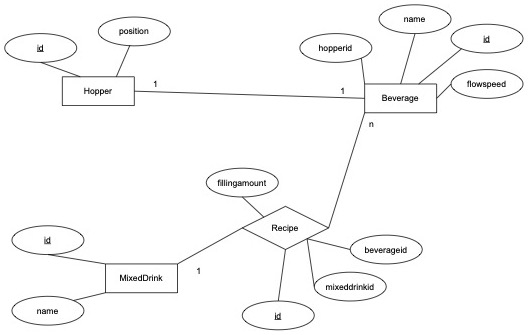
\includegraphics[width=120mm]{content/figures/database.jpg}
        \caption{Database structure \label{fig:database}}
    \end{figure}


\section{Micro Controller}

    For the microcontrollers, the choice fell on the  \textit{RP2040} \cite{rp2040}. With the help of the \textit{Raspberry Pi Pico SDK} \cite{sdk} it is relatively easy to write programs in the C language for it. The peripherals include 2 UARTs for easy communication with the stepper drivers. 

    The controllers were used in the form of the \textit{Tiny 2040} \cite{tiny2040}. The \textit{Tiny 2040} is a development board that complements the \textit{RP2040} with a USB-C connector and easily accessible IO pins.


\section{Stepper driver}

    \textit{TMC2209s} were selected as stepper drivers because they offer a UART interface that provides reliable communication and allows a wide range of settings. 
    Up to four drivers can be connected simultaneously to one UART master. In addition, they operate almost silently. \cite{tmc2209}

    For communication with the stepper drivers, a \textit{TMC2209} library \cite{tmcLibrary} and a \textit{Serial-over-UART} implementation, both originally written for the \textit{Arduion IDE} in \textit{C++}, were rewritten in \textit{C}.

\section{Mototor}



\section{Limit Switch}

    A limit switch lets current through when it is closed and not when it is open. Therefore, it can be detected when a specified physical limit is reached.

\section{LED}



\section{Power Supply}



\chapter{Evaluation}


\chapter{Conclusion}



% Appendix chapters to be put here. They will be enumerated with capital letters 
% if you  did not change the \documentclass options.
\begin{appendix}


%\include{appendix_chapterA}
\end{appendix}
%Ende Anhang

%Bibliography
% We strongly recommend to use bibtex to manage your bibliography. It helps you
% structure your references and helps avoiding missing important data for a correct
% quotation. If you have no other idea jabref (http://jabref.sourceforge.net/)
% might be a good idea (Jave runtime environment needed).
% This style is good to use in german master thesis'. You need to have activated
% \usepackage{bigerm} above.
% For english documents just use apalike.
\bibliographystyle{geralpha}

% to finally announce where your bibliography is stored use
\bibliography{content/references/references}
% it is also possible to have several files separated by comma. 
%Bibliographie Angaben mit \bibliography{}

%!TEX root=../../Vorname_Nachname_Diplomarbeit.tex
%pagenumbering{null}

\ 

%clearpage
\cleardoublepage

\ 


\pagestyle{empty}

\textbf{Versicherung an Eides Statt}\\

Ich versichere an Eides statt durch meine untenstehende Unterschrift,
\begin{itemize}
\item[-] dass ich die vorliegende Arbeit - mit Ausnahme der Anleitung durch die Betreuer - selbstständig ohne fremde Hilfe angefertigt habe und
\item[-] dass ich alle Stellen, die wörtlich oder annähernd wörtlich aus fremden Quellen entnommen sind, entsprechend als Zitate gekennzeichnet habe und
\item[-] dass ich ausschließlich die angegebenen Quellen (Literatur, Internetseiten, sonstige Hilfsmittel) verwendet habe und
\item[-] dass ich alle entsprechenden Angaben nach bestem Wissen und Gewissen vorgenommen habe, dass sie der Wahrheit entsprechen und dass ich nichts verschwiegen habe.
\end{itemize}
Mir ist bekannt, dass eine falsche Versicherung an Eides Statt nach \S 156 und \S 163 Abs. 1 des Strafgesetzbuches mit Freiheitsstrafe oder Geldstrafe bestraft wird.
\vfill
Duisburg, \today\\
$\overline{\parbox{4.8cm}{(Ort, Datum)}} ~~~~~~~~~~~~~~~~~~~~~~~~~~~ \overline{\parbox{7cm}{(David Lewakis)}}$


\end{document}
%%% Local Variables:
%%% mode: latex
%%% TeX-master: t
%%% End:
